\section{Módulo de Reconhecimento}

	O Módulo de Reconhecimento é responsável pela identificação dos usuários no ambiente utilizando a face como característica biométrica. A face foi escolhida pois ela permite um reconhecimento não intrusivo, como mencionada na Seção~\ref{sec:biometria}. A detecção e o reconhecimento são feitos em imagens de usuários que são passadas pelo Módulo de Rastreamento. Tais imagens são compostas somente pela região em que o usuário se encontra, como mostrado na Figura~\ref{fig:users-img}.

	Basicamente, o processo de reconhecimento é realizado pelas seguintes etapas e ilustrado na Figura~\ref{fig:processo-reconhecimento}:

		\begin{figure}[htb]
			\begin{center}
				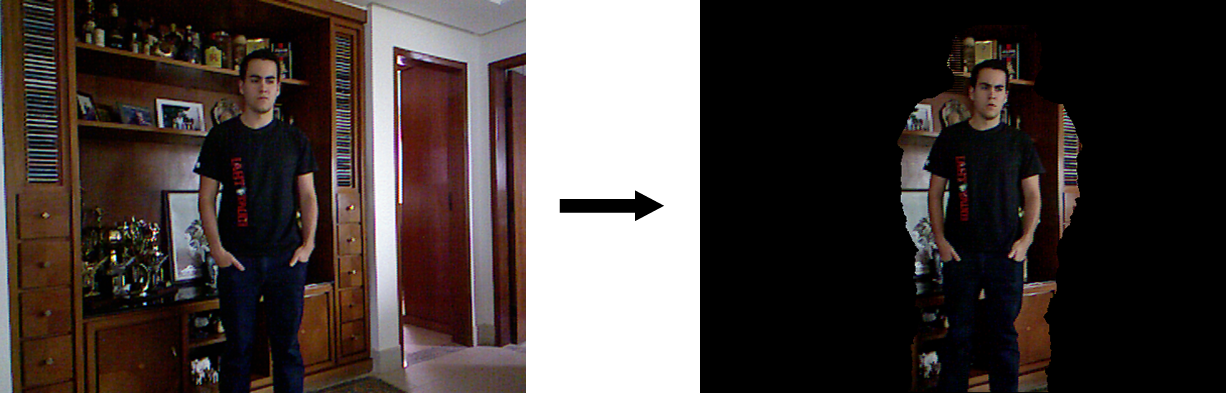
\includegraphics[scale=0.3]{figuras/4.ProblemaEProposta/users-img.png}
			\end{center}
			\caption{Exemplo de uma imagem composta somente pela região em que o usuário se encontra.}
			\label{fig:users-img}
		\end{figure}

		\begin{enumerate}
			\item Obtém a imagem de entrada correspondente a imagem formada somente pelo usuário cujo reconhecimento foi requisitado.
			\item Pré-processamento da imagem: a imagem é convertida em escala de cinza.
			\item Realiza detecção facial na imagem. Caso nenhuma face seja encontrada, retorna ``vazio''. Vale ressaltar que no máximo uma face pode ser encontrada nesta imagem.
			\item Processamento da imagem: uma nova imagem é criada recortando a região da face encontrada, a imagem, então, é redimensionada e equalizada criando assim um padrão de tamanho, brilho e contraste nas imagens aumentando a acurácia do reconhecimento.
			\item Reconhecimento facial com \textit{Eigenfaces} é realizado.
			\item Retorna o nome da face ``mais parecida'' e a confiança do reconhecimento.
		\end{enumerate}

		\begin{figure}[htb]
			\begin{center}
				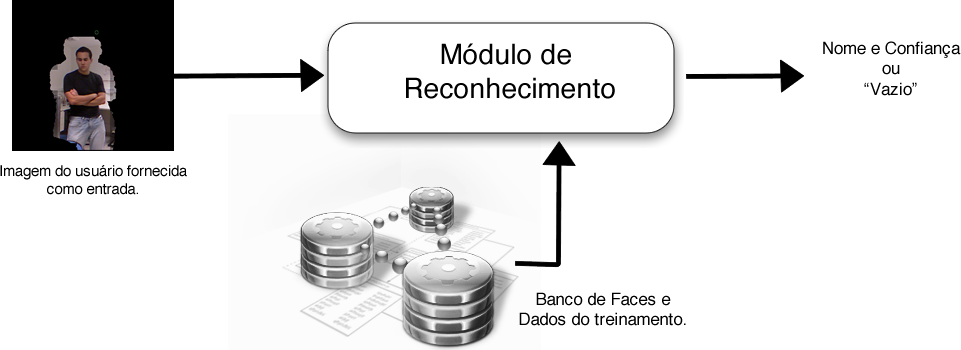
\includegraphics[scale=2.0]{figuras/4.ProblemaEProposta/reconhecimento-simples.png}
			\end{center}
			\caption{Módulo de Reconhecimento do Sistema TRUE.}
			\label{fig:processo-reconhecimento}
		\end{figure}

	% O Módulo de Reconhecimento é dependente do de Rastreamento. Ele ficará ocioso
	% até que chegue uma requisição de reconhecimento de um determinado usuário. A
	% Seção~\ref{sec:rastreamento-reconhecimento} explica mais detalhadamente a
	% relação entre os dois módulos.

	\subsection{Pré-processamento e Processamento da Imagem}
		
		As etapas de processamento das imagens permitem criar um padrão nas mesmas aumentando a acurácia do reconhecimento. No Sistema TRUE as etapas de processamento consistem em converter a imagem em escala de cinza, recorta-la, redimensiona-la e equaliza-la criando, assim, um padrão de cor, tamanho, brilho e contraste nas imagens.

		A Figura~\ref{fig:greyscale} exemplifica uma imagem normal de uma face,
		depois a mesma convertida em escala de cinza e equalizada O
		Apêndice~\ref{apend:processamento} mostra trechos de código em linguagem C
		que implementam tais etapas.

		\begin{figure}[htb]
			\begin{center}
				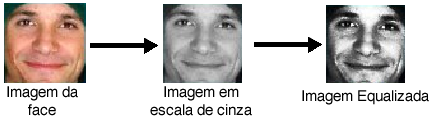
\includegraphics[scale=0.7]{figuras/4.ProblemaEProposta/greyscale.png}
			\end{center}
			\caption{Exemplo de uma imagem de face normal, em escala de cinza e equalizada. Adaptada de~\cite{shervin}.}
			\label{fig:greyscale}
		\end{figure}

	\subsection{Detecção Facial}

		A detecção facial foi desenvolvida utilizando o método \textit{Viola-Jones}~\ref{ref:viola-jones}. Um método que pode ser utilizado para construir uma abordagem de detecção facial rápida e eficaz~\cite{violajones} em tempo real. Além disso, este método é implementado pela biblioteca \textit{OpenCV} (\textit{Open Source Computer Vision}) onde bons classificadores em cascata de características \textit{Haar} são fornecidos.

		Basicamente, o processo de detecção facial procura por uma face em uma imagem pré-processada. Para realizar detecção facial utilizando o método \textit{Viola-Jones} é necessário a utilização de um classificador em cascata, como mencionado na Subseção~\ref{subsec:reconhecimento}. Portanto, entre os diversos classificadores em cascata presentes na biblioteca \textit{OpenCV}, foi utilizado o classificador \textit{haarcascade\underline{ }frontalface\underline{ }alt.xml}, um classificador treinado para detectar faces frontais em imagens.

		% A Figura~\ref{fig:diagrama-deteccao} mostra o fluxo básico do processo de detecção de faces no Sistema TRUE.
		% 	\begin{figure}[H]
		% 	\begin{center}
		% 		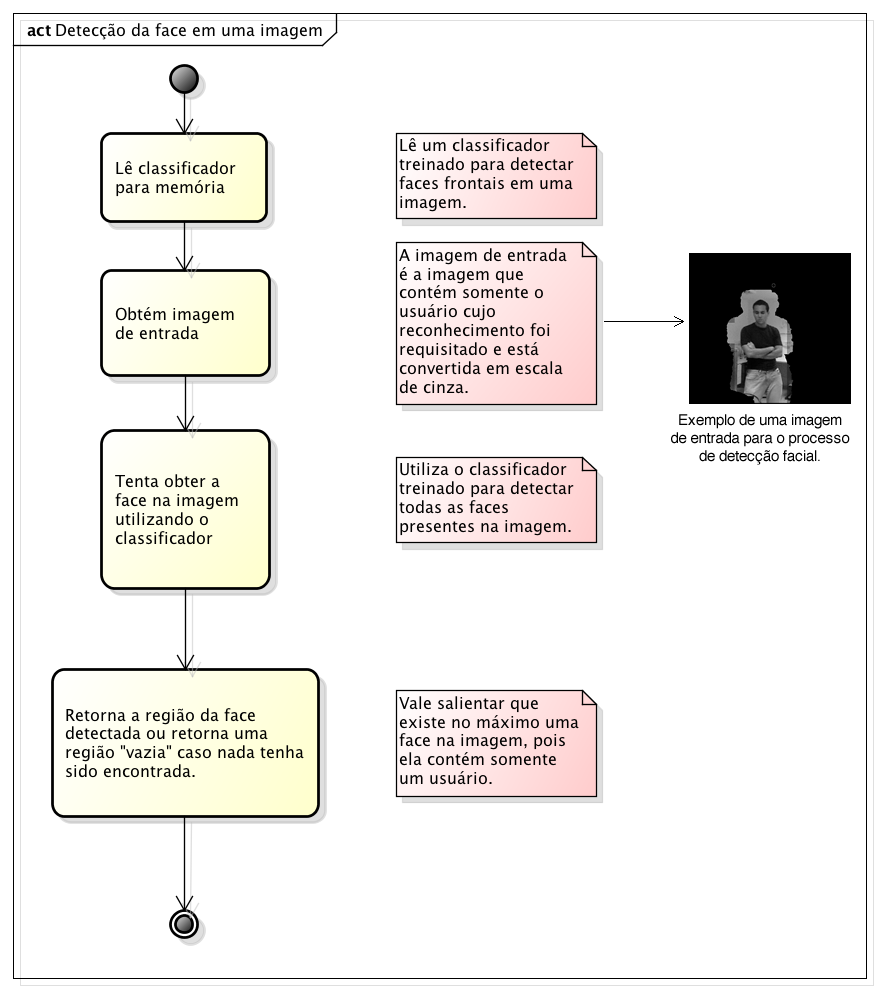
\includegraphics[scale=0.5]{figuras/4.ProblemaEProposta/diagrama-detectar-face.png}
		% 	\end{center}
		% 	\caption{Fluxo de execução do processo de detecção facial no Sistema TRUE.}
		% 	\label{fig:diagrama-deteccao}
		% \end{figure}

		O processo de básico de detecção de faces no Sistema TRUE possui as seguintes etapas:

		\begin{enumerate}
			\item Lê um classificador treinado para detectar faces em uma image.
			\item Obtém a imagem de entrada. Tal imagem é composta somente pelo usuário, como mostrado na Figura~\ref{fig:users-img}, cujo reconhecimento foi requisitado, além de estar em escala de cinza.
			\item Utilizando o classificador, tentar obter uma face na imagem.
			\item Retorna a região da face detectada ou retorna ``vazio'' caso nenhuma face tenha sido encontrada. Vale salientar que existe no máximo uma face na imagem, pois contém somente um usuário.
		\end{enumerate}

	\subsection{Reconhecimento Facial com \textit{Eigenfaces}}

		O reconhecimento facial foi desenvolvido utilizando
		\textit{Eigenfaces}~\ref{sec:reconhecimento}. Uma técnica bastante
		satisfatória quando utilizada sobre uma base de dados (faces) relativamente
		grande, permitindo ao sistema inferir, das imagens suas principais
		características e, partindo delas, realizar o reconhecimento das imagens
		utilizando um número bastante reduzido de cálculos~\cite{artigo-eigenface},
		permitindo, assim, um reconhecimento em tempo real.

		A base de dados utilizada no Sistema TRUE é formada por imagens no formato PGM (\textit{Portable Gray Map}) com tamanho de 92x112 pixels e em escala de cinza. A base é composta por um banco de faces de alunos de Ciência da Computação da Universidade de Brasília e por um banco de imagens de faces da Universidade de Cambridge~\cite{cambridgeFaceDb}, mostrado na Figura~\ref{fig:cambridgeFaceDb}. Este último, é formado por imagens de faces de 40 pessoas diferentes. Para cada pessoa, existem 10 diferentes imagens tiradas em diferentes épocas, com diferentes condições de iluminação, com diferentes expressões faciais (olhos abertos e fechados, sorrindo e não sorrindo, entre outros) e com diferentes detalhes faciais (óculos, sem óculos). 

		\begin{figure}[htb]
			\begin{center}
				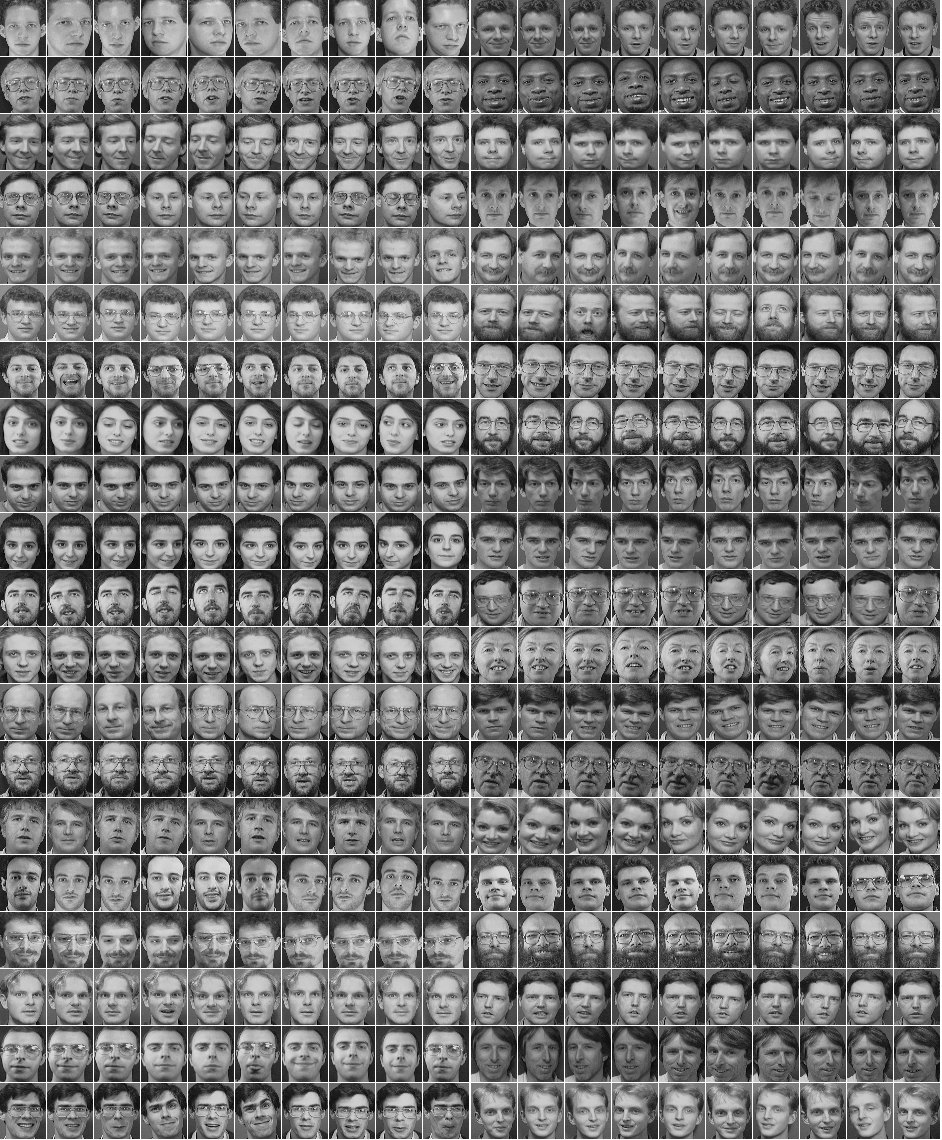
\includegraphics[scale=0.4]{figuras/4.ProblemaEProposta/cambrigdefacedb.png}
			\end{center}
			\caption{Banco de imagens de faces da Universidade de Cambridge~\cite{cambridgeFaceDb}.}
			\label{fig:cambridgeFaceDb}
		\end{figure}

		A Figura~\ref{fig:diagrama-reconhecimento} mostra o fluxo básico do processo de reconhecimento facial no Sistema TRUE.

			\begin{figure}[htb]
			\begin{center}
				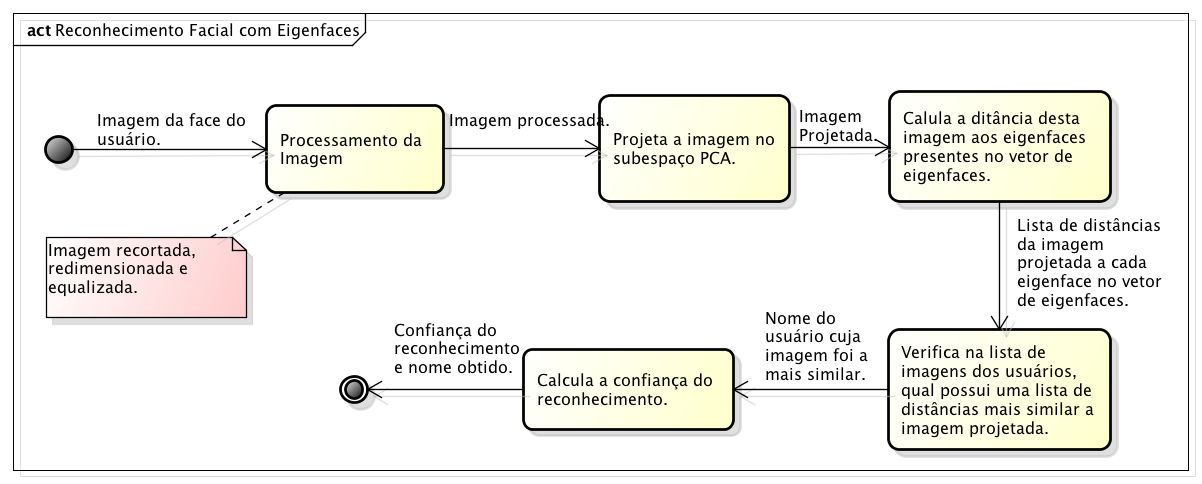
\includegraphics[scale=0.5]{figuras/4.ProblemaEProposta/diagrama-reconhecimento2.png}
			\end{center}
			\caption{Fluxo de execução do processo de reconhecimento facial no Sistema TRUE.}
			\label{fig:diagrama-reconhecimento}
		\end{figure}

		% A primeira etapa consiste na leitura dos dados de treinamento. Esses dados são compostos pela lista dos nomes e imagens das faces dos usuários cadastrados no sistema, pelo vetor de \textit{Eigenfaces}, pela \textit{Eigenface} média e pelos \textit{eigenvalues}.

		% Uma das etapas intermediárias consiste no cálculo da distância entre a imagem projetada no subespaço PCA aos eigenfaces. Inicialmente, o cálculo desta distância era feito utilizando distância euclidiana, porém não apresentava bons resultados em algumas condições. Portanto, este cálculo passou a ser feito utilizando distância Mahalanobis. Contudo, ela também não apresentou bons resultados em alguns casos. Então, alguns testes foram feitos utilizando as duas distâncias de maneira conjunta: uma imagem só é tida como reconhecida quando o resultado das duas distâncias apontarem para a mesma identidade. Com isso, houve uma melhora significativa dos resultados.

		Uma das etapas intermediárias consiste no cálculo da distância entre a imagem projetada no subespaço PCA aos \textit{eigenfaces}. Inicialmente, o cálculo desta distância era feito utilizando distância Euclidiana. Contudo, testes foram realizados com alguns usuários, em que o sistema realizava 20 tentativas de reconhecimento de usuários, e os resultados não foram satisfatórios. Portanto, os mesmos testes foram realizados utilizando distância Mahalanobis. Porém, os resultados também não foram satisfatórios. Então, os mesmos testes foram feitos utilizando as duas distâncias de maneira conjunta: uma imagem só é tida como reconhecida quando o resultado das duas distâncias apontarem para a mesma identidade. Com isso, houve uma melhora significativa dos resultados. Os resultados destes testes são mostrados na Tabela~\ref{tab:distancias}, onde fica claro a melhora dos resultados quando se utiliza ambas distâncias. Nessa tabela, os nome Pessoa1, Pessoa2, Pessoa3, são nomes dados as pessoas cujas fotos estão presentes no banco de imagens de faces da Universidade de Cambrige~\cite{cambridgeFaceDb}.

		\begin{table}[H]
		\begin{center}
			\caption{Resultados do teste de reconhecimento feito com o usuário Danilo utilizando as diferentes distâncias.}
			\label{tab:distancias}
			\begin{tabular}{|c|c|c|c|c|c|c|c|}
				\hline & \bf Danilo & \bf Pedro & \bf Ana & \bf Pessoa1 & \bf Pessoa2 & \bf Pessoa3 & \bf Desconhecido\\
				\hline \bf Euclidiana & 45\% & 40\% & & 5\% & 5\% & 5\% &\\
				\hline \bf Mahalanobis & 40\% & & 15\% & 35\% & 10\% & &\\
				\hline \bf Ambas Distâncias & 75\% & & & & & & 25\%\\
				\hline
			\end{tabular}
		\end{center}
	\end{table}

		A última etapa consiste no cálculo da confiança do reconhecimento. 
		
		% TODO: Explicar como se calcula.

		% A confidence of 1.0 would mean a god match, and a confidence of 0.0 or negative would mean a bad match. But beware that the confidence formula I use in the code is just a very basic confidence metric that isn't necessarily too reliable, but I figured that most people would like to see a rough confidence value. 
